\chapter{Optical pumping of an atom laser}
\label{OpticalPumping}
\graphicspath{{Figures/OpticalPumping/}{Figures/Common/}}

The results presented in this chapter have been published in \citet{Robins:2008,Doring:2009}.

\section{Motivation}

The development of the continuous-wave optical laser was a significant advance over the first pulsed ruby laser. The continuous-wave optical laser opened up many applications. The atom laser is a very promising source for both precision measurement and fundamental physics.

The replenishment process can be divided into two critical components: a delivery system for filling an atomic reservoir with ultracold atoms and a pumping mechanism for irreversibly and continuously transferring atoms from the reservoir to the laser mode.

The technical requirements on both parts of the replenishment system are stringent. Nonetheless, recent experiments have demonstrated that a delivery system for atoms is feasible and possible. \citet{Chikkatur:2002qa} showed that Bose-condensed atoms could be periodically transported over large distances using a moving optical dipole trap. Further experiments with transport, based on interference of two counter-propagating lasers, have shown that dipole trapping techniques could be extended to provide continuous delivery of atoms \citep{Schmid:2006}. Magnetic guiding systems for ultracold atoms may also provide a path to future delivery systems \citep{Lahaye:2004,Greiner:2001,Greiner:2007}.

The realisation of the pumping mechanism for a continuous atom laser has proved more problematic. There are four critical requirements that are difficult to satisfy experimentally. First, the atoms should enter the laser mode continuously and coherently, that is, with the phase and amplitude of the lasing condensate. Thus, atoms must make a transition that is Bose-stimulated by the atomic lasing mode. The second requirement is that the pumping process is irreversible. It requires coupling to a reservoir. There are two reservoirs available, the empty modes of the electromagnetic field accessible via a transition from an excited atomic state, or the empty modes of the atomic field accessible via evaporation. For a high-coherence atom laser, the lasing mode must be a pure condensate with a significantly smaller thermal fraction, making evaporation-induced pumping a difficult possibility for the production for a highly coherent continuous atom laser. The third requirement is that the pumping system must be compatible with a continuous replenishment mechanism. This suggests strongly that there be a physical separation between the source and the lasing condensates. A physical separation with a stimulated transition between the source and the lasing mode isolates the lasing mode from phase kicks and heating that would result either as a necessary consequence of the replenishment system (for example in the replenishment system demonstrated by \citet{Chikkatur:2002qa} where condensates are merged) or as a consequence of an imperfect delivery system. Finally, the fourth condition on a pumping system is that it should be possible to continuously output-couple atoms from the laser mode into a beam, while the pumping mechanism is operating.

The two possibilities for reservoirs to supply the irreversibility necessary for the proper operation of a pumped atom laser (Bose-Einstein condensate) are considered in this chapter and the next. In this chapter, pumping an atom laser using interactions mediated by light is considered. In this case the reservoir providing the irreversibility are the vacuum electromagnetic modes into which light is scattered by the pumping process. \chapterref{KineticTheory} considers the alternate possibility of using atomic s-wave scattering interactions to mediate the pumping process with evaporation to make the process irreversible.

\hrule

Previous work on light-BEC interactions. Rayleigh/Raman superradiance, EIT, CARL, and the rest of that list that I had.


\section{Pumping mechanism}

\begin{figure}
    \centering
    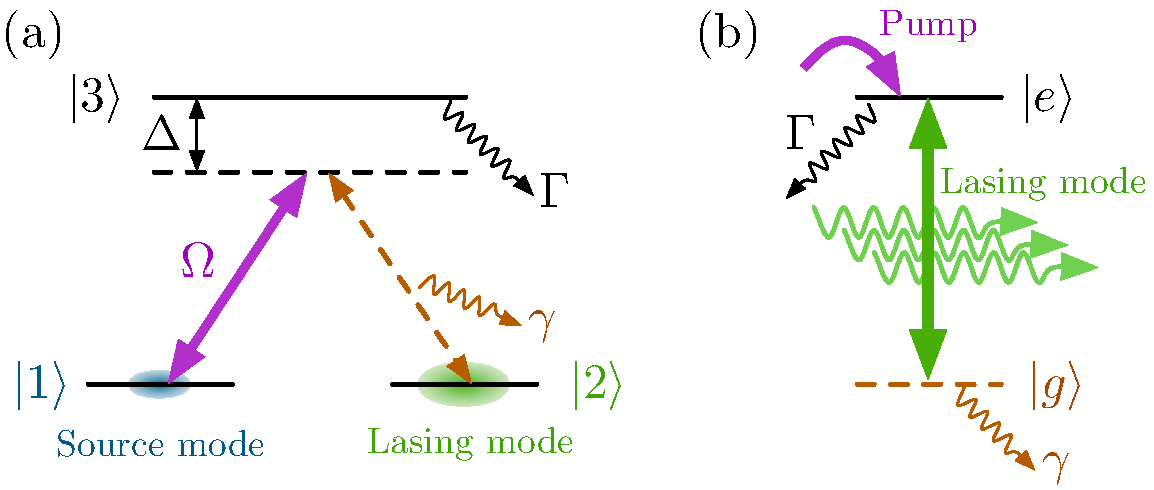
\includegraphics[width=14cm]{LambdaModel}
    \caption{FIXME: This is not a caption. Comparison of considered atom laser pumping scheme (a) and typical optical laser pumping scheme (b).\label{OpticalPumping:LambdaModel}}
\end{figure}

The optical pumping process under investigation in this chapter is illustrated in \figureref{OpticalPumping:LambdaModel}(a).  In this process atoms in the source mode are driven by a laser into an excited state from which they can decay into the lasing mode (the condensate).  Although there is no laser driving this second transition ($\ket{3}\leftrightarrow\ket{2}$), the decay of atoms into the lasing mode is not spontaneous emission in the usual sense.  The emission process is \emph{atomically}-stimulated by the large occupation of the lasing mode in the same way that the transition may be \emph{optically}-stimulated even in the absence of any population in the atomic state into which the atom decays.

The final decay of an atom into the lasing mode in \figureref{OpticalPumping:LambdaModel} resembles standard \emph{optical} laser schemes [see \figureref{OpticalPumping:LambdaModel}(b)] in which the roles of atoms and light are reversed.  In an optical laser an atom in the excited state is stimulated to emit into the ground state by the resonant photons in the laser cavity.  Once the atom has emitted, it decays rapidly into other internal states with rate $\gamma$ significantly limiting reabsorption from the $\ket{g}$ state.  A similar process occurs in the proposed optical pumping scheme in which the photon emitted as the atom decays  leaves the system rapidly preventing reabsorption.  The loss of photons from the system is represented by the decay of the optical mode with rate $\gamma$ in \figureref{OpticalPumping:LambdaModel}(a).

This similarity between the proposed atom laser pumping mechanism and the usual optical laser pumping mechanism is clearly illustrated by considering the Hamiltonian coupling the excited and ground atomic states in \figureref{OpticalPumping:LambdaModel}
\begin{align}
    \hat{H} &= \hbar \epsilon \left(\hat{a}_e^\dagger \hat{a}_g \hat{a}_\text{ph} + \hat{a}_g^\dagger \hat{a}_\text{ph}^\dagger \hat{a}_e  \right),
    \label{OpticalPumping:TwoLevelAtomHamiltonian}
\end{align}
where $\epsilon$ is a real coupling constant, the $\hat{a}_e$, $\hat{a}_g$, and $\hat{a}_\text{ph}$ are annihilation operators for the atomic excited state, atomic ground state and photon mode respectively.  The rotating wave approximation has been made in obtaining this Hamiltonian, assuming that the optical mode is not detuned from the atomic transition by a large fraction of the frequency difference between the two states.  

The Hamiltonian \eqref{OpticalPumping:TwoLevelAtomHamiltonian} describes both the atom- and optical-laser pumping mechanisms, the difference in the mechanisms being in the occupations of the various states.  If the system is initially in a state with $N_e$ atoms in the atomic excited state, $N_g$ atoms in the atomic ground state and $N_\text{ph}$ photons in the optical mode, the amplitude for an atom in the excited state to emit a photon is
\begin{align}
    \bra{N_e-1, N_g + 1, N_\text{ph} + 1} \hat{H} \ket{N_e, N_g, N_\text{ph}} &= \hbar \epsilon \sqrt{N_g+1} \sqrt{N_\text{ph}+1} \sqrt{N_e}.
\end{align}
This emission process can therefore be stimulated either by photons ($N_\text{ph} > 0$) or by atoms ($N_\text{g} > 0$).  It would also be possible for the emission to be stimulated by both photons \emph{and} atoms, although in this case the amplitude for the absorption process would be non-zero
\begin{align}
    \bra{N_e+1, N_g - 1, N_\text{ph} - 1} \hat{H} \ket{N_e, N_g, N_\text{ph}} &= \hbar \epsilon \sqrt{N_e+1} \sqrt{N_\text{ph}} \sqrt{N_g}.
\end{align}
It is for this reason that it is desirable in an optical laser to have $N_g \approx 0$, and in the proposed atom laser pumping scheme to have $N_\text{ph} \approx 0$.

Variations of the atom laser pumping scheme presented in \figureref{OpticalPumping:LambdaModel}(a) have been proposed before (FIXME: cite stuff) for the production of BEC without the use of collisional evaporation and its consequent losses.  There are two difficulties with these schemes, the first is that only a small fraction of the 





There have been two difficulties with these schemes, the first is that only a small fraction of the 


The atom laser pumping scheme presented in \figureref{OpticalPumping:LambdaModel}(a) has been proposed before (FIXME: cite stuff) for the production of BEC without collisional evaporation and its consequent losses.  There are two difficulties with these schemes, the first is that 


using `all-optical' means\footnote{Originally this additionally meant without using a collisional evaporation process, however more recently `all-optical BEC' has included the use of collisional evaporation in optical traps \citep{Barrett:2001}.} using thermal atoms in the source mode.  


There are two difficulties with these schemes, the first is that 


Two difficulties with this, firstly reabsorption (also an issue here that will be discussed at length later) and the Franck-Condon factor




Now it would be appropriate to talk about this mechanism having been proposed before.




As the optical transition between the excited atomic state and the lasing mode is not driven by a laser, the phase of the photons emitted is determined by the relative phase between the source and lasing modes; the direction of population transfer does not depend on the phase difference between these two modes.  Indeed, provided the emitted photons left the system sufficiently quickly the proposed pumping mechanism could also transfer thermal atoms in the source mode to the lasing mode the random phase differences between these modes being carried away by the emitted photons.



The emitted photons in the optical pumping mechanism 




As the optical transition between the 


The direction of the population transfer between the source mode and the lasing mode does not depend on the relative phase between the two 

in the absence of collisions

The population transfer between the source mode and the lasing mode does not depend on 


Phase difference between the source and lasing mode. The present scheme does not require coherent atoms, discuss differences.

Need to discuss past, similar proposed pumping mechanisms.  At the moment, the proposal is very similar to that considered previously by others.  The main difference being that a coherent source is being considered.  Discuss how this is a significant difference.



The interchangeability of atomic 


Something about the use of coherent atomic source implying that we cannot simply treat the Bose-stimulation as an accelerated spontaneous emission.  Though this only occurs in the detuned case.  Not true, also occurs in the resonant case. Only becomes obvious in a multimode model.

FIXME:  We need a note here about retaining the effects of coherence.



The primary difference between the present work and that which has come before is the use of coherent atoms as the source driving the pumping mechanism.  While this is certainly not ideal, it is not unrealistic provided that the pumping mechanism is independent of the phase difference between the source and lasing modes (unlike the work of \citep{Savage:1998nx}).




The pumping mechanism under investigation in this chapter is illustrated in \figureref{OpticalPumping:LambdaModel} and bears some similarity to EIT, Raman outcoupling, and Rayleigh/Raman superradiance.  In this mechanism, a coherent sample of atoms in the source mode are driven by an optical field into an excited state from which they can decay into the target mode.  The decay of atoms into the target mode cannot simply be viewed as a spontaneous emission process, as the target mode contains a macroscopic occupation.  Stuff and nonsense.


Similar mechanisms have been proposed before (FIXME: Add citations, see Santos:2001ve and Savage:1998nx).

a coherent sample of atoms in a source mode are optically excited into 


The pumping mechanism under investigation in this chapter is illustrated in \figureref{OpticalPumping:LambdaModel} and is very similar to EIT, Raman outcoupling, and Rayleigh/Raman superradiance.  


Reabsorption of spontaneously emitted light.  Go with Simon's plan.  There is basically no other way around it.  Say in what limit the approximation is valid.  Point out that this topic will be revisited at the end of the chapter.  More sophisticated treatments are necessary to consider the case of thermal atoms for the source. 


The scheme for a pumped atom laser is illustrated in ...





We revisit this discussion of spontaneous emission towards the end of the chapter (FIXME: Insert reference once the section is written).


Use an optical transition to drive atoms into the target condensate.  You might initially think that this process is spontaneous emission and therefore not coherent, but the process is stimulated emission.  It's just that it is stimulated \emph{atomically}, not optically.  This is a really cool idea.  We can talk about the equivalence of these two different simulation mechanisms, and how you can have both simultaneously.  It's all in the amplitudes for the processes.  Part of the issue is how to get the atoms into the excited state to be able to do the entire transfer process coherently.  STIRAP-type transitions are an obvious possibility.  The trouble becomes that to operate STIRAP continuously, the timing of the pulses must translate to the spatial shape of the `pulses'.  This implies $0 \hbar k$.

$2 \hbar k$ might work in the detuned case.  Note that a STIRAP-type process may not be needed as the photons are leaving the system making the process irreversible.  So is STIRAP really needed? As long as the photons leave quickly (but not too quickly), it should work.  The analogous process would be having the atoms in the target state rapidly decay to another state. Then you could irreversibly drive the source atoms into the other states.  In fact, this is how optical lasers operate.  This case relies on the fact that the emitted photons are not seeded.

In the experimental realisation of the scheme, there are two alternative geometries for the pumping ($0\hbar k$ or $2 \hbar k$).  The difference in how the experiment is performed is in fact negligible, so this creates some issues about differentiating the two.  

We note at this point one important point: what about the resonant emitted photons (if they are resonant)?

\section{The continuous pumping experiment}
\label{OpticalPumping:ContinuousExperiment}

The experiment was performed by \emph{Nick Robins}, \emph{Cristina Figl} and \emph{Matthew Jeppesen}.

Describe that delicate, fragile experiment that produced some positive results.  Note that the pumping light went through many ND filters, so the intensity of that light was very low.  Stupid amounts of baffling (I was confused the first time I heard that term), waiting until the dead of night, etc.  25-30\% pumping efficiency after outcoupling the entire source condensate. Yay! Absence of heating! Yay!

Two condensates, outcoupling from the upper condensate to form a freely-propagating atom laser in the $F=2$, $m_F=0$ state.  The atoms in this atom laser then absorb a photon and emit one (in which direction) being stimulated by the lower condensate.  Simultaneous with this pumping mechanism, one can outcouple from the lower condensate.  The net effect is a quasi-continuously pumped atom laser.  Not exactly a continuously-pumped atom laser, but the pumping mechanism is a significant part of the process, and this experiment represents a significant step forward.

\section{Simple single-mode model}
\label{OpticalPumping:SingleModeModel}

This is the simple model that exhibits the Quantum Zeno effect, multiple equilibrium states and a bunch of other interesting physics.  We have to motivate the driving term for the optical field, but other than that, the system is fairly well behaved.  Using this model it can be shown that the pumping should work in both the resonant and detuned cases.  Note that one of the things that this model does not consider is the loss of atoms before they reach the region in which they overlap with the target condensate. Neither can this model represent STIRAP-type processes. Unless you model them in a temporal domain, but STIRAP is well understood anyway.

The model is a simple $\Lambda$-type scheme, but where one of the optical fields is `spontaneous'.

\section{Multimode model (in 1D)}
\label{OpticalPumping:MultimodeModel}

The 1D model is based on the Maxwell-Schrödinger equations.  One of the technical difficulties is the fact that we must be able to solve in the case that light is travelling in opposite directions simultaneously.  It is not an issue analytically, the equations are well-defined.  The trouble is solving the system self-consistently.  The equations as posed are stiff and are best treated by implicit algorithms, but the best we have are half-arsed semi-implicit algorithms. Better yet would be to use a finite-element method and treat the cross-propagation properly, but I'm lazy.  The other issue is that the frequency of the light is usually known \emph{a priori}.  That is not the case for at least one of the modes in this system.  We therefore need to use some fancy tricks in order to get around that issue.  However, any detunings should not be too large.

Apart from the Maxwell part of the system of equations, everything else is fairly standard.  Except of course for the 1D reduction itself.  We'll call it a `central-line' approximation.

Somewhere in here we need to mention the adiabatic elimination and what kinds of terms it gives rise to.  And in what limit the approximation is valid (even close to resonance).

We need to talk about the other assumptions made in the model.  The assumption that spontaneous emission is negligible.  There is a question about how the 1D approximation affects the Franck-Condon factor, and the relationship between that and spontaneous emission.

Now is a good time to consider $0 \hbar k$ vs $2 \hbar k$ and resonant vs detuned in a simplified model in which things can be controlled (two overlapping modes in the same trap and where $k \rightarrow 0$). The important difference being the \emph{geometry}.

\subsection{3-level model}

This is a simplified model that contains only a small number of levels so that it is easier to keep track of what is going on.  We assume that we can outcouple directly from the $F=2$, $m_F=2$ trapped condensate to the $F=2$, $m_F=0$ state. This isn't realistic, but it is useful to simplify the whole process.  I believe the excited $F'$ manifold was also reduced.  With this simplified model we can investigate resonance vs detuned.  I seem to recall some crazy interesting physics where we had atom transfer back to the \emph{source} condensate in the $0 \hbar k$ configuration in the detuned case.  I believe it was all about phase differences and stuff.  If you look at the equations from the zero-dimensional model, the direction of transfer depends on the phase of a couple of terms, so it can go either way.  For the resonant case, the atoms were definitely transferred to the \emph{target} condensate, as desired.  Also, try as we might, it was not possible to get the $2 \hbar k$ resonance working efficiently.  Too much loss on the way.  Though I don't remember what happened in the detuned $2 \hbar k$ case.

This simplified 1D model contains all of the important physics related to the pumping process.  The delivery of atoms to the target condensate is simplified, and some of the optical transitions are removed.  This model is partly to validate the simple zero-dimensional model including some multimode dynamics, and also to try to get some basic agreement with the experiment before moving on to a more complete description in a later section.

\subsubsection{Comparison with experiment}

We consider both the $0\hbar k$ and the $2\hbar k$ resonance and find that we are able to get reasonable agreement with the experiment in the $0\hbar k$ limit, although it was incredibly fiddly to maximise the transfer.  The $2\hbar k$ resonance was dominated by loss of atoms as they travelled between the source and target condensates.  Although it must be stated that the experimentalists had a good idea of their detunings from rf spectroscopy.  The detunings did indicate that the required conditions for the $0 \hbar k$ resonance were not present.  They were however appropriate for the $2 \hbar k$ resonance, which was the one originally hoped for.  I can't remember, but I wanted to reproduce the experimental rf-spectroscopy data theoretically for some reason.

Anyway, things look great. So why don't we add more realism and see what we get? Maybe we can get even better agreement!

\subsection{5-level model}

The 5-level model is like the 3-level model, but including the full $F=2$ manifold.  Also, the full $F'=1$, $F'=2$ and $F'=3$ excited state manifolds are included before adiabatic elimination.  This model is designed to illustrate the full physics of the situation.  

\subsubsection{Comparison with experiment}

The theory in this case is completely defeated by the crazy mode shape of the $F=2$, $m_F=1$ level.  As this mode is trapped, it oscillates about the lower condensate.  If the intensity of the light is too low, these atoms block the pumping light from even reaching the target condensate and the $F=2$, $m_F=0$ atoms.  If the intensity of the light is too high, the atoms undergo spontaneous emission before they even reach the lower condensate, and you don't get any $F=2$, $m_F=0$ atoms.  If you try for something in the middle, the Franck-Condon factor between the $F=2$, $m_F=0$ atoms and the condensate is very small due to the crazy mode shape of the $F=2$, $m_F=1$ atoms from which the $F=2$, $m_F=0$ atoms are outcoupled.

In short, the 5-level model shows no pumping at all. But not because of something fundamental with the atom transfer process, but rather due to boring technical details about providing the atoms in the appropriate state and mode.  Besides, 1D models are very poor approximations to 5-level systems on timescales beyond the time for the $F=2$, $m_F=1$ atoms to reach the centre of that trap as the atoms will focus at the origin in the tight trapping dimension significantly increasing the density there over what would be seen in a purely 1D model.

\subsection{The pulsed pumping experiment}

The pulsed pumping experiment had the same basic set up as the continuous experiment, but instead a pulse of atoms (the \emph{transfer pulse}) was outcoupled from the upper condensate.  As this pulse was outcoupled over $\unit[100]{\micro s}$ (or whatever time it was) the issue of detuning essentially doesn't arise.  The Fourier width of the outcoupling pulse is large enough to essentially outcouple a copy of the condensate into the different Zeeman levels.  This transfer pulse was allowed to fall a variable delay time before pulsing on the same pumping light used in the continuous experiment.  The transfer pulse was finally allowed to fall further before imaging to determine the number of atoms remaining in the transfer pulse.  Due to the vastly different densities of the condensate and the transfer pulse, it is impossible to simultaneously measure the size of each.  Moreover, as the transfer pulse is significantly smaller than the target condensate, it was impossible to determine the number of transferred atoms to the target condensate.

\subsubsection{Theory / Experiment comparison}

We have good agreement with the loss of atoms out of the transfer pulse, which suggests that the $2 \hbar k$ resonance is workable, although it must be realised that operating a pulsed experiment is fundamentally different to the operation of the continuous experiment.  One model for the operation of the continuous experiment suggests that a process like STIRAP is occurring in the spatial domain instead of the usual temporal domain.  By operating the experiment in the pulsed regime, we are able to cause this process to occur in the temporal domain again, allowing access to the $2 \hbar k$ resonance.  Regardless, there are some questions that remain unanswered.  While we have good agreement on the transfer of atoms \emph{out} of the pulse, the experiment has no information about the transfer of atoms \emph{into} the condensate.  For this question, we can only rely on the theory.  In this case, the theory suggests that there should be a significant number of photons emitted spontaneously within the lower condensate.  A single one of these photons should cause significant (observable) heating of the lower condensate.  The issue is that no such heating is observed.  We are left scratching our heads on this issue (see next section).

\section{Discussion / Outlook}

This is where we say that we have reasonable evidence to say that we know what is going on in the transfer of atoms to the lower condensate, but a pretty poor explanation for what happens afterwards.  It is precisely this latter process that was thought to prevent optical pumping of condensates, and so the fact that the expected heating has not been observed is of great interest.  We can speculate wildly as to the origin of this absent heating, including BAR and quantum-mechanical collective effects due to the coherence of the atom laser.  Fundamentally, it seems to me that the notion of spontaneous emission is broken when the emission is occurring in the centre of a BEC.  On the edge, it probably mostly works.  In the centre, I'm not entirely convinced.

\section{Conclusion}

The conclusion I have been thinking of at the moment is along the following lines.  There have been three parts to the optical pumping process: (i) the delivery of atoms in an appropriate state to the condensate being pumped; (ii) the transfer of those atoms to the condensate being pumped; and (iii) the behaviour of the emitted photons within the pumped condensate.  This present chapter has aimed to understand part (ii) of this process.  Ideally we would also like to understand (iii) as it appears that there is some very interesting physics occurring in this part of the process, however we have fallen short of this goal.  By contrast process (i) is a technical detail of getting atoms to the lower condensate with an appropriate mode.  There are several methods that could be used for this process, and there are a number of arguments why the models used in this chapter are unsuitable for fully describing process (i).  Technical details are of course important, but not of fundamental importance.  And it has been the fundamentally important processes that we have aimed to investigate in the present chapter.
